\documentclass{mprop}
\usepackage{graphicx}

% alternative font if you prefer \usepackage{times}

% for alternative page numbering use the following package and see documentation
% for commands \usepackage{fancyheadings}


% other potentially useful packages \uspackage{amssymb,amsmath}
\usepackage{url}
%\usepackage{fancyvrb} \usepackage[final]{pdfpages}

\begin{document}

%%%%%%%%%%%%%%%%%%%%%%%%%%%%%%%%%%%%%%%%%%%%%%%%%%%%%%%%%%%%%%%%%%%
\title{Is Technical Debt Real?}
\author{Ovidiu Popoviciu}
\date{18th December 2017}
\maketitle
%%%%%%%%%%%%%%%%%%%%%%%%%%%%%%%%%%%%%%%%%%%%%%%%%%%%%%%%%%%%%%%%%%%

%%%%%%%%%%%%%%%%%%%%%%%%%%%%%%%%%%%%%%%%%%%%%%%%%%%%%%%%%%%%%%%%%%%
\tableofcontents
\newpage
%%%%%%%%%%%%%%%%%%%%%%%%%%%%%%%%%%%%%%%%%%%%%%%%%%%%%%%%%%%%%%%%%%%

%%%%%%%%%%%%%%%%%%%%%%%%%%%%%%%%%%%%%%%%%%%%%%%%%%%%%%%%%%%%%%%%%%%
\section{Introduction}\label{intro}

\begin{itemize}
	\item What is technical debt?
	\item What are its applications?
	\item Why is it important?
\end{itemize}

Technical debt - definition \\
What impact does TD have on development?\\
How much work effort is wasted on new features on a codebase impacted with
technical debt?\\
Why is it difficult to define such a measure? \\
If such a measurement is known, how could it be managed? \\
What are the advantages of quantifying technical debt interest in the form work
effort? \\

Goal-Question-Metric approach is a good framework for breaking down research
work. (TODO: add citation here)

Goal-Question-Metric approach:
\begin{itemize}
	\item Goal: \textbf{Analyze} project feature implementations \textbf{with
		      the purpose of} identifying extra work \textbf{from the viewpoint of}
	      software engineers and project manager \textbf{in the context of}
	      technical debt management.
	\item RQ1: Can technical debt interest for a team be predicted for each
	      sprint?
	\item RQ1.1: What was the difference (delta) in the estimated work effort
	      for a feature and the practical work effort due to technical debt?
	\item RQ1.2: What is the measurement of TD in the affected modules across
	      change sets?
	\item RQ1.3: How does work effort delta vary with the magnitude of
	      technical debt?
	\item RQ2: What are the development patterns surrounding feature
	      lifecycle?
	\item RQ2.2: At what checkpoint in development is technical debt reduction
	      (refactoring)  most prominent?
\end{itemize}

Problem statement: Has the student analysed the problem, stated it clearly, and
justified its importance?

%%%%%%%%%%%%%%%%%%%%%%%%%%%%%%%%%%%%%%%%%%%%%%%%%%%%%%%%%%%%%%%%%%%
\section{Background Survey}

\subsection{Study Design}

\begin{itemize}
	\item Technical debt definition
	\item Types of TD - focus on code and design debt
	\item Measurement of principal and interest
	\item Measurement of work effort and team productivity
	\item Management of TD
\end{itemize}

\subsection{Definition, Perspectives and Types}
\label{section:def}

% Ward Cunningham - WyCash Portfolio Management System TODO: expand the
% definition from the paper.
Technical debt is a metaphor termed by Ward Cunningham, in his famous report on
the WyCash Portfolio Management System in 1993 \cite{Cunningham1993}. In the
report, Cunningham mentioned that "\textit{shipping first time code is like
	going into debt.}" and that as the system evolves new features would become more
and more difficult to implement. This phenomenon was due to feature-rich
projects being shipped to customers early but poorly written with little or no
consideration to quality and to future work.

\begin{figure}
	\centering
	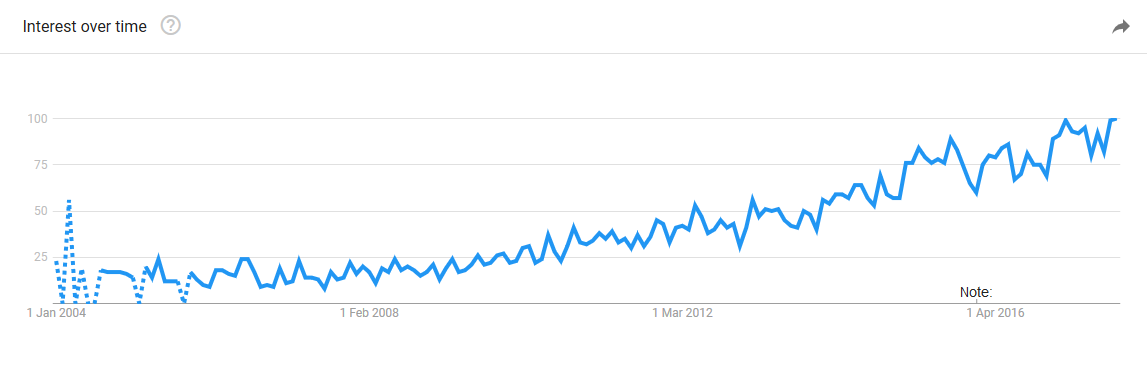
\includegraphics[width=\linewidth]{visualisations/TD_trend.png}
	\caption{Technical Debt Trend from 2004 to Present}
	\label{fig:td-trend}
\end{figure}

% MTD 2010
The metaphor was ignored for a long time, until the late 2000s, when more and
more studies started to explore the phenomenon and possible management
processes. A figure of the popularity of Technical Debt from 2004 to present can
be seen in Figure \ref{fig:td-trend}, information provided by Google Trends
\cite{GoogleTrends}. Thus, the first workshop on managing technical debt took
place in 2010, where an initial research agenda was proposed for the future of
software engineering field. Since then, workshops have been held every year,
which consisted seminars, presentations and brainstorming sessions on aspects
such as definition \cite{Kruchten2012} \cite{Theodoropoulos2011}
\cite{Schmid2013}, identification \cite{Ernst2012}, measurement
\cite{Letouzey2012} \cite{Curtis2012} \cite{Nugroho2011} \cite{Zazworka2011}
\cite{Fontana2012} \cite{Bohnet2011}, management \cite{Guo2011}
\cite{Zazworka2011Prioritise} \cite{Seaman2012} to industry case studies
\cite{Lim2012} \cite{Morgenthaler2012} \cite{Codabux2013} \cite{Holvitie2014}
\cite{Klinger2011}.

% from metaphor to theory and practice TODO: add citation to industry case
% studies
The definition of technical debt relies heavily on the perspective of the viewer
and her responsibility within the socio-technical environment. Developers view
technical debt as a list of software quality issues and correlate it with lack
of time to implement features "\textit{properly}" \cite{Codabux2013}. Product
managers and stakeholders view at it as a strategy, a way to defer quality work
for fast work in order to satisfy certain business requirements, such as Time to
Market (TTM). In practice, these two perspectives are widely different, with
developers prioritising "invisible" code perfection whilst management focusing
on rapid development of "visible", selling point features. Kurchten et al.
\cite{Kruchten2012} defined technical debt as technological gaps between
development teams and management, where a gap is the evolution of a context
specific to a decision taken in the past. These gaps might have been decisions
that seemed correct when the decision was taken however, with the passing of
time, the initial decision incurred debt within the project. For example, there
is no tool that predicts what frameworks and languages will exist in the future
or how to implement features by considering future unknown requirements. As a
consequence, the authors state that technical debt is not the collection of code
quality violations within the results of static code analyzers but, a phenomenon
which is heavily reliant on present and future project evolution.


% from a stakeholder's perspective
However, most strategic decisions on the future evolution of the project come
from management. Unfortunately, stakeholders might not have knowledge of the
metaphor of technical debt, its current measurement and whether it impacts costs
of development. Their main focus of increasing business value through the
addition of visual features, rather than looking for investment in the quality
of the software being produced. As a result, new features are prioritised and
pressured on being delivered as early and as quickly as possible. These types of
issues affect the \textbf{extrinsic quality} of software and are "visible". For
example, an extrinsic quality characteristic is usability. Deferring user
experience work and ignoring user interface bugs might force users of the system
to find "ways around" certain tasks. The result is negative impact in user
productivity and the general usefulness of the product. Extrinsic
characteristics are important to the business as they are considered "sell
points" of the product. On the other hand, \textbf{intrinsic quality}
characteristics of software are the low-level issues such as code smells,
best-practices violations that might slow down development of new features
unless refactoring processes are applied. Theodoropoulos et al.
\cite{Theodoropoulos2011} considered that intrinsic and extrinsic software
quality characteristics are interdependent and deferring quality maitainence in
one area may affect other areas of quality. For example, improper data
validation in the business logic layer of the system, may impact downstream
components, such as user interface, and produce bugs within the system.


% on the limits of td metaphor TODO: define principal and interest
Although the use of finance terms may simplify technical characteristics of
software quality in the dialogue between development teams and stakeholders, the
analogy breaks down as studied by Schimd et al. \cite{Schmid2013}. In their
study, the authors had identified shortcomings in the financial metaphor
established by Ward Cunningham \cite{Cunningham1993} and found points where it
breaks down. In the financial domain, debt is a well known arrangement between
two parties where one party borrowes a fixed amount of money from the other
party \cite{debt-investopedia}. The most well known types of debt are loans,
where the terms of the arrangement dictate that the amount of money borrowed
must be paid back in full after a fixed period of time, along with fixed
interest payments paid annually.

Schmid et al. \cite{Schmid2013} has identified three major points where the
analogy breaks down:
\begin{itemize}
	\item \textit{Unit of measurement}. In finance there is a clear unit of
	      monetary measurement through the use of international currencies. In
	      contrast, technical debt does have a standard unit of measurement
	      defined. There are many tools (TODO: add citation of paper tools
	      here) that provide a single, quantified and aggregated measure of
	      the amount of time it takes for software quality issues to be
	      resolved. Additionally, very few of these tools quantify the
	      consequences of neglecting refactoring and the improvement in
	      quality characteristics. The issue of measurement puts a dent into
	      the shared vocabulary between development and stakeholders as
	      mentioned by a number of software practioners from industry case
	      studies (TODO: add industry case study citation here).
	\item \textit{Fixed time period}. On the one hand, debt arrangements have
	      a fixed \textit{maturity date}, where the debt must be paid back. On
	      the other hand, software quality issues do not a have a time limit
	      and may be kept in the product until they are resolved. Fixing these
	      items relate to paying back the "loan" taken on their creation. Such
	      issues may never be paid back if not needed to, resulting in an
	      increased cost-value ratio.
	\item \textit{Fixed interest}. A loan arrangement additionally consists of
	      fixed interest payments measured as a percetange of the loan value,
	      paid on an annual or bi-annual basis. The interest compensates for
	      the risk taken by the lender and encourages the loanee to pay back
	      quickly as possible in order to avoid paying back too much interest.
	      In reality, there is no such thing as fixed interest dependant on a
	      single factor in technical debt. Interest is difficult to quantify
	      as a matter of principal, and the amount of interest paid after a
	      period of time depends on future work.
\end{itemize}
Under these circumstances, what is considered "good structure" or "clean code"
is also heavily influenced to future development since future decisions
influence cost impact. As a consequence, no system is \textit{debt free} and
thus fixing every code violation would be an act of gold plating. Additionally,
what is the value of paying back this debt if the product is competitive and the
customers are happy \cite{Lim2012}?

% martin fowler - td quadrants
In Martin Fowler's famous article \cite{TDMartin}, he described this type of
future debt as \textbf{inadeverted-prudent} debt. Over time, a project that was
"clean" may find that after a period of time that the initial approach taken
might not have been the best. He considered that developers learn on the job to
perfect their craft as time passes. The four quadrants refer to the types of
technical debt that one might encounter in a software project given the approach
taken by the development team. It was one of the four quandrants he defined, as
shown in Figure \ref{fig:td-quandrants}.

\begin{figure}
	\centering
	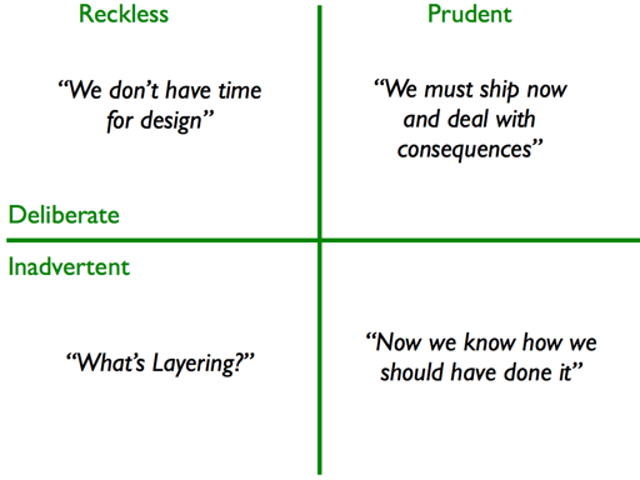
\includegraphics[width=0.5\linewidth]{visualisations/TD_quadrants.png}
	\caption{Martin Fowler's Technical Debt Quadrants}
	\label{fig:td-quandrants}
\end{figure}


% unhedged call option
An alternative metaphor of technical debt \cite{UnhedgedCallOption}, described
bad code using finance terms in a similar fashion, but through a different
financial intrument called a call option.
\textit{An option is a financial derivative that represents a contract sold by
	one party (the option writer) to another party (the option holder). The contract
	offers the buyer the right, but not the obligation, to buy (call) or sell (put)
	a security or other financial asset at an agreed-upon price (the strike price)
	during a certain period of time or on a specific date (exercise date).}
\cite{option-investopedia}. A call option gives the right to buy while a put
option gives the option holder the right to sell. In software engineering, if a
feature is hacked up quickly using bad code and never touched again, then the
project had reaped the rewards. The option "was not called". However, if a new
feature were required that would be influenced by the quick and dirty work
implemented earlier, then the requirement would be more expensive to fulfill. In
this case, the option "has been called".


% conclusion
Defining software quality issues as a financial metaphor helps bridge vocabulary
shortcomings between developers and stakeholders. It helps management understand
current software development risks and encourages ways for managing these risks
as they are created. TODO: make sure to write down the exact definition As
Cunningham \cite{Cunningham1993} had written, technical debt may be used as a
strategy in order to meet business expectations however, if not repaid promptly
it could bring entire corporations to a standstill.

% types of TD
Initially, technical debt has solely focused on the internal quality issues of
systems developed. Such issues could be code smells, code violations and
duplicate or complex code. However, multiple types of debt have been
"discovered" spanning the entire socio-technical environment.
% TODO: maybe add a description for all types of debt but only focus on code
% debt
A mapping study, conducted by Li et al. \cite{Li2015}, have analysed 94 papers,
overall dating 1992-2013, and have found 10 types of technical debt being
studied: requirements debt, architectural debt, design debt, code debt, test
debt, build debt, documentation debt, infrastructure debt, versioning debt and
defect debt. The most prominent type of debt studied was code debt, followed by test,
architectural, design and documentation debt.

% architecture debt is the worst - industrial case study
However, in an industrial case study \cite{Codabux2013}, developers considered that
architectural debt is the most difficult to adress, due to complexity and change
impact on project. Major architectural decisions are not taken in a vaccuum and
thus requires group meetings with other developers, software architects and
product managers. The time to reach a consensus on how to approach such changes
improve the cost of managing architectural debt.

% technical debt is "technical"
A few of the authors have considered that the metaphor of technical debt should
only apply to the low-level, internal quality characteristics such as code,
design, test, architectural debt rather than process gaps such as inadequate
quality assurance \cite{Theodoropoulos2011} \cite{Nugroho2011}. Thus the word
"technical". However, business process gaps may negatively affect projects and
incurr technical debt as a result.

%%%%%%%%%%%%%%%%%%%%%%%%%%%%%%%%%%%%%%%%%%%%%%%%%%%%%%%%%%%%%%%%%%%
\subsection{Identification and Measurement}

% What are the causes of code TD?

Technical debt may impede future development and delivery of new features if not
managed appropriately \cite{Cunningham1993}. Cunningham's statement was
validated by a number of authors by looking at the most "notorious" code smells
\cite{Fowler1999} and their impact on software projects.

Olbrich et al. \cite{Olbrich2009} studied the impact of two code smells, God
class and Shotgun Surgery, on change proneness of class entities and size of
changes within two open source systems, namely Apache Lucene and Apache Xerces.
They gathered data on the number of smells in the systems over revisions and the
distribution of changes on classes suffering from these two smells. The authors
concluded that large systems are more prone to increase the number of code
smells as it evolves over time and particularly, that classes suffering from the
God class smell are 4 to 5 times more change prone than other classes. However,
the study was conducted only on open-source systems and the results might not pe
applicable to commercial software. Additionally, due to limitations of the tool
used to identify code violations, only public Java classes have been analysed.

In a similar study, Fontana et al. \cite{Fontana2012} studied the impact of
removing code smells on code quality metrics. The authors looked at three common
smells: Data class, God class and Duplicated Code. Additional goals were to find
out which code smell incurs the most TD and whether their impact is related to
the domain of product being built. The metrics impacted are cohesion, coupling
and complexity. Proper refactoring practices were applied for each smell whilst
the quality metrics were re-evaluated to assess their impact. The results showed
that refactoring of one code smell may provide benefits for one or more metric
qualities but may negatively impact others. Interestingly, they had found that
the Data Class smell and God class smells frequency may be domain-dependent.

An exploratory study by Khomh et al. \cite{Khomh2009} empirically analysed the
impact of 29 code smells on the change sets of 9 releases of two open source
systems. They had confirmed the results of the previous studies that code smells
increase the number of changes that software undergoes during its evolution.
Additionally, they had found that classes containing more than one code smell
are more change prone than other classes. Moreover, they found a possible cycle
of repairing smells and introducing new ones between releases.

An interesting idea from all authors \cite{Olbrich2009}, \cite{Fontana2012} and
\cite{Khomh2009} stated that not all code smells have the same consequences on
the code base. A code smell may have been deliberately introduced due to the
nature of project domain. For example, in the case of a system that uses
computer vision algorithm and techniques might be prone to an increased
cyclomatic complexity and God class smells.

% prioritisation by severity - interest probability
Thus, Charalampidou et al. \cite{Charalampidou2017} introduced a study that
assessed the interest probability of code smells, where the interest probability
is the probability of a code smell to introduce extra changes in future
development. Interest probability was calculated by counting the frequency of
each code smell and how it correlates with the change proneness of the module
where it resides. The smells studied were Long Method, Conditional Complexity,
and Duplicated Code. The results showed that code duplication has the highest
interest probability due to the number of changes required to maintain future
development. Additionally, high cyclomatic method complexity increases amount of
changes.

% prioritisation on context
Additionally, prioritising code smells with the highest severity might not be
suitable if the context in which the smell resides will not be referenced in the
future. Therefore, Sae-Lim et al. \cite{Sae-Lim2016} looked at prioritising code
smells according to development context to support a \textit{prefactoring}
stage, where developers clean up code before development of new features. The
authors calculated a value for each code smell, called the \textit{Context
	Relevance Index}, based on a list of issues from the project's issue tracker and
the change descriptors of commits in the project version control. The results of
their preliminary study returned a list of ranked code smells to be targetted as
a prefactoring step to implementation. This type of prioritisation may be more
practical in time constrained projects.

% conclusion of measurement TODO: add citation here 
Code smells are technical debt items and increase future development and
maintainance costs. Industry case studies have shown that TD items are more
likely to be addressed if made visible by developers within the project's issue
tracker. However, from the perspective of a project manager, it is of importance
to know how much effort the team will put into technical debt reduction and
whether there is an associated business value with this investment. Hence,
subsequently to the identification stage of code smells, there must exist a
measurement stage of the amount of work effort technical debt will introduce to
be resolved and the consequences on productivity over time if the team keeps
hold of the code violations.

% How to quantify code smell impact?

% introduction
Identification and prioritisation are two of the most important stages when
dealing with technical debt. Making technical debt items such as code smells
visible has been recommended by industry practitioners \cite{Lim2012}
\cite{Codabux2013}. However, participants have struggled to find a way to
measure technical debt and its cumulative effect over time. This is a
particularly important aspect of project managers responsibility when planning
new work for the team. Whilst developers are concerned with the health and
quality of the codebase, managers are responsible with balancing work by keeping
developers and stakeholders happy.

Specifically, a technical debt item raises two important questions:
\begin{itemize}
	\item How much effort does it take to repair it?
	\item What are the consequences of holding on to it?
\end{itemize}

Answering these two questions through a quantified measure is the key to a
proactive management of technical debt. The measure depicting the cost of paying
back the debt at the present time is called the \textit{principal} whilst the
extra cost of development when keeping hold of items is called
\textit{interest}. Unfortunately, there is no standardised method, due to
difficulties managing complexities of quantifying work effort and development
costs. However, a number of studies have appeared over the years that look at
methods for calculating principal and interest of technical debt items.

An interesting paper by Bohnet et al. \cite{Bohnet2011} proposed a tool to
bridge the gap between development teams and corporate managers, by exposing
internal system quality through the use of \textit{software maps}. A software
map is a hierarchical 2D/3D view of software artefacts, each represented
visually through properties such as colour, texture and size; each representing
a property of quality: cyclomatic complexity, lines of code and nesting levels.
Such a visualisation provides both developers and managers with points of
fragility where possible bugs may arise and highlights areas of work to address.
However, the visualisation is technical and might be difficult to convey to
stakeholders. Additionally, there is no way to calculate the principal and
interest of the quality issues.

% sqale method for measuring technical debt
Letouzey et al. \cite{Letouzey2012} proposed a different method, called the SQALE
method. The goal was to create a standardised, language-agnostic framework for
assessing the quality of source code by deriving measures for code
characteristics and calculating an overall measure of technical debt. The
framework proposed consisted of four concepts:
\begin{itemize}
	\item Quality Model - defines internal properties of code through a
	      structured three-layer hierarchy (characteristic, sub-characteristic and
	      requirement). For example, a characteristic is maintainability,
	      sub-characteristic is readability and the requirement is no commented
	      code. The hierarchy is defined as all requirements could be converted into
	      actionable steps. Each requirement defines a remediation index (cost to
	      repair code violations) defined in time, work or capital units.
	\item Analysis Model - measurement of the distance between the current
	      state of the application and the \"optimized\" quality target.
	\item Indices - these are the values that represent the costs of paying
	      back debt.
	\item Indicators - provide a visual representation of technical debt indices
	      through ratings.
\end{itemize}
The indices were calculated by summing up the principal of each code violation
and aggregating up into the sub-characteristics and further to the
characteristics of the Quality Model. The technical debt index is provided
through the aggregation of all the characteristics in the Quality Model.
Although the framework provides a good measurement of technical debt from the
principal of code violations, there is no calculation of interest if TD items
are not reduced and, additionally, it does not take into consideration
architectural debt issues. Subsequently to their study, the method was
implemented in SonarQube, which is a continuous code quality tool.

Curtis et al. \cite{Curtis2012} summarized the results of a language agnostic
study on a huge database (365M lines of code) of software projects across 10
industries which provided a formula for estimating the principal of TD items.
The authors used CAST's Application Intelligence platform to statically analyse
source code, using 1200 rules of coding "best practices". They identified code
violations by analysing source code and aggregated the results into quality
characteristics, or \textit{health factors}. Scores from each health factor were
aggregated on a scale of 1 (high risk) to 4 (low risk). The total principal was
estimated by a formula with three parameters: number of problems, time required
for each fix and the cost of fixing the issue. Unfortunately, the methodology
did not support calculation of holding on to code issues. The authors concluded
that estimating the interest incurred by a TD item was difficult since might be
multiple hidden factors which influenced the results. The term works well with
the phenomenon since stakeholders think of software quality in terms of
business.


Nugroho et al. \cite{Nugroho2011} looked at defining an empirical formula for
quantifying principal and interest. The authors had completed an empirical
analysis of 44 projects within the Software Improvement Group (SIG) using TUViT
software quality assessment method for collecting relevant metrics: lines of
code, code duplications, etc. The had defined technical debt from an opposite
perspective, as the changes needed to bring a system from its current quality
state to the "ideal" quality. They considered technical debt to be equivalent to
a measurement of repair effort (RE). Calculation of this measure required the
number of lines of code that need to changed, the estimate work effort of
rebuilding the feature from scratch and a margin of error. The interest was also
derived from the extra cost spent on maintainance monthly and yearly, modelled
against the current state of quality. The conclusions were that the formulas for
principal and interest could be used in quantifying important business
information such as Return on Investment (ROI). However, due to the nature of
ranking system quality (scale of 1-5), it would be a challenge to get ROI right.


Another interesting study was conducted by Singh et al. \cite{Singh2014}, where
technical debt interest payments were calculated by monitoring of development
effort and code comprehension. The proposed approach monitors time spent by
developers in classes with known TD items, detected initially by static analysis
tools. They integrated a tool within the Integrated Development Environment of
developers and gathered information of class visits, development session times
within the class. The interest was calculated as the difference between time
practically spent in classes and the ideal time spent. The results showed that
developers tend to spend more time in classes containing TD items than others.
However, the study was conducted with the input of one developer over a period
of 9 months. Additionally, estimating the ideal time spent on development is a
challenging task due to multiple personal factors such as level of project
knowledge, familiarity of environment and programming language, etc. A possible
solution would be to study development time from a more coarse-grained approach,
from a feature or release level.

Gomes et al. \cite{Gomes2011} studied the correlation between software
evolution, defect occurrence and work effort deviation at the release level. The
authors extracted data from multiple documentation sources such as test plans,
project plan, weekly reports, project source code, and emails. Using this data,
they could derive important team information on change, effort, quality, test
and size of the system. They measured extra work effort by subtracting the
estimated work time and total work time. Although information at the release
level offers project managers an idea of work effort deviation, it does not show
at a granular level what defects slow down development of a new feature and
where the team should focus their refactoring activities.

% Tools?

These types of measurements are useful for project managers when making
decisions as to what percentage of work on an interation to be assigned on
refactoring. To keep up with a constantly changing system, there are software
quality tools used in industry that analyse source changes, highlight possible
fixes and some have automatic refactoring features.

% experience report on code smell detection tools
Fontana et al. \cite{Fontana2011} compiled an initial report on code smell
detection tools and their experience on the analysis of multiple versions of an
object-oriented Java project. The goal of their study was to contrast the
performance of these tools in relation with known code smells in the source
code. These tools were: Jdeodorant, PMD, iPlasma, InFusion, StenchBlossom. There
were numerous code smells initially detected in the project including God Class,
Data Class, Feature Envy, Brain Method, etc. Their methodology was to apply
analysis on multiple versions of an object-oriented project, with all code
smells known beforehand. They have found not all tools identify all the code
smells in the project and some had different names for the same code smell.
Additionally, some tools shared the same metrics and identified the same
collection of smells, whereas others had widely different results.

% Technical Debt Indexes Provided by Tools
Unfortunately, the experimented tools had only the ability to identify code
violations and link them to the source code. No tool had features on quantifying
software quality and no mention of a global technical debt measurement. Other
tools have been implemented which provide such aggregated values. They provide
the ability to calculate the "quantity" of technical debt as well as a total
estimated amount of effort for its reduction. However, each tool takes into
consideration different information sources and calculates the overall TD
measurement in a different way since there exists no standard method on
aggregating such a complex phenomenon into a single value.

Hence, a new study by Fontana et al. \cite{Fontana2016}, had looked into the 5
code quality tools that provide these features, with the goal to understand how
they calculate technical debt, what sources of information they take into
account and what features they are missing. The study looked at the following
tools:
\begin{itemize}
	%TODO: add link to pages
	\item \textbf{CAST}. Defines technical debt cost by taking both principal
	      and interest into consideration. The principal is calculated by the
	      severity, time and cost to fix structural flaws. Interest is then computed
	      by assuming that a business will resolve a fixed percentage of high, medium
	      and low severity items, times the cost of labour set at 75\$ per hour.
	\item \textbf{InFusion}. Calculates a measurement, Quality Deficit Index,
	      which summarizes the level of quality of a system. It takes into account all
	      design flaws of a source code, each described by negative influence on best
	      practices, level of granularity (method or class level) and smell severity.
	\item \textbf{Sonargraph}. The distinction from the rest of the tools is
	      that developers can set a defined initial architecture and Sonargraph can
	      find deviations from that architecture at the level of system, project and
	      build. Additionally, the tool generates two Structural Debt measurements, an
	      index related to the sum of all dependencies needed to be cut and a cost
	      measurement calculated from the index multiplied by a time factor.
	\item \textbf{SonarQube}. A continous code quality tool that uses a large
	      amount of rules for good coding practices to find code violations. The
	      resulting code violations are aggregated into software quality characterstic
	      factors which then compute a Technical Debt Index. The index is expressed in
	      the of work effort required to fix all issues. Rules and costs may be
	      modified to support customised business requirements (available in the
	      commercial version). It implements the SQALE method of measuring technical
	      debt \cite{Letouzey2012}.
	\item \textbf{Structure101}. Tool specialised in architectural issues of the
	      codebase, with metrics on multiple levels of granularity such as method,
	      class, package and project level.
\end{itemize}

The authors have provided summarized tables that describe all the tools and
their purpose nicely. The two tables are available in Figure \ref{fig:tools-tables}.

\begin{figure}
	\centering
	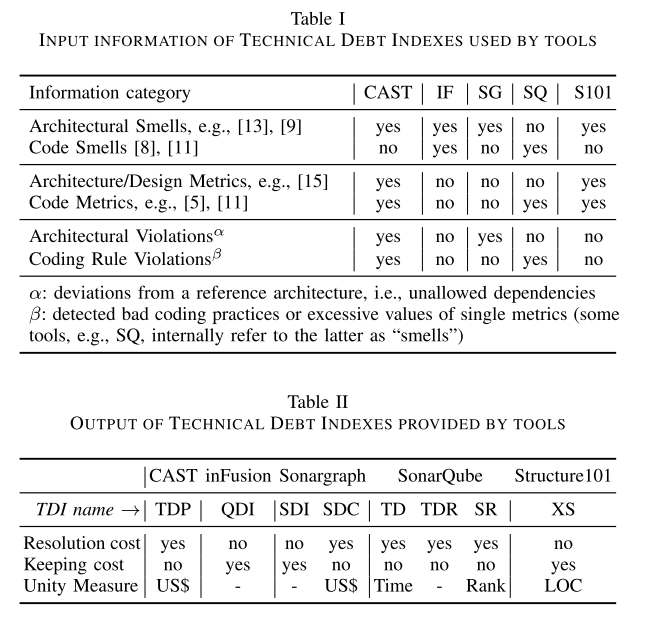
\includegraphics[width=0.5\linewidth]{visualisations/tools-table.png}
	\caption{Summary of tools provided by Fontana et al.}
	\label{fig:tools-tables}
\end{figure}

Unfortunately, there is no standard method of measuring the total technical of a
system. This is due to the complex nature of the metaphor and one cannot capture
all its complexities into a single tool. Therefore, there is no single best tool
for this purpose, as all take into consideration different sources for metric
computation and it all comes down to the requirements of the team looking to
increase the level of software quality.

%%%%%%%%%%%%%%%%%%%%%%%%%%%%%%%%%%%%%%%%%%%%%%%%%%%%%%%%%%%%%%%%%%%
\subsection{Management}

Although tools provide managers with an approximate measure of quality of the
code base, there is a danger in associating technical debt with the results of
software quality tools. As mentioned in Section \ref{section:def}, there
are numerous types of technical debt that may have a negative impact on the ROI
of the business. For example, code quality tools cannot predict that the
requirements gathering phase was not completed appropriately or that build debt
is affecting infrastructure costs \cite{Morgenthaler2012}.

Additionally, a study by Martini et al. \cite{Martini2017} showed that the
overall impact of technical debt at the project level is not same as the sum of
all technical debt items. They assessed four projects and interviewed both
project managers and developers on their perspective of the impact, on a scale
from 1 to 10. Although the interviewees had multiple backgrounds and were
consulted on many development factors (reduced development speed, bugs incurred
by TD, extra costs, frequency of issues, spread in system, users affected,
etc.), the results showed that there are other complexities affecting the
project.

Technical debt should be used as a strategy for quick development of features in
order to satisfy an immediate business requirement such as TTM. From an
industrial case study \cite{Lim2012}, a developer described TD as follows:
"\textit{Technical debt is a balance between software quality and business
	reality}". Industry practitioners from the same study have acknowledged that
numerous business requirements have forced them to incur debt. Unfortunately,
business requirements and decisions are difficult to foresee due to constant
market deviations, such as the appearance of a new competitor or a new
technology.

Therefore, technical debt is difficult to predict. However, it is recommended
that once debt is incurred, it should be made visible \cite{Lim2012}
\cite{Codabux2013} \cite{Morgenthaler2012}, and paid back as early as possible.
Cunningham \cite{Cunningham1993} describes it best: "\textit{The danger occurs
when the debt is not repaid. Every minute spent on not-quite-right code counts
as interest on that debt. Entire engineering organizations can be brought to a
stand-still under the debt load of an unconsolidated implementation,
object-oriented or otherwise.}".

Fortunately, project management methodologies such as Agile and its associated
practices have proved to help reduce and manage technical debt
\cite{Holvitie2014} \cite{Trumler2016}. In particular, Test Driven Development (TDD),
following coding standards, refactoring, continuous integration, collective code
ownership and pair programming have been considered to help tackle technical
debt.

From a project manager's perspective, technical debt must be managed at cost
level by iteration. How many resources should the team invest in technical debt
reduction over the next sprint? What issues should the team tackle first and
what will the benefits be?

Guo et al. \cite{Guo2011} suggested that technical debt should be managed
similar to a financial portfolio perspective by encouraging each item to be
viewed as an investment. Debt items would take on the role of assets, with the
same goals: maximize return and minimize risk. The decision framework would be
based on historical metrics of all TD items to decide which ones to keep and
which ones to pay back. However, the approach is difficult to achieve in
practice due to limitations of the metaphor \cite{Schmid2013}.

Seaman et al. \cite{Seaman2012} proposed four ways to aid in this decision
making:
\begin{itemize}
	\item Cost-Benefit Analysis. The technique is based on principal, interest
	probability (the probability that other work will be more expensive),
	interest amount and their associated value (high, medium, low). Using these
	it would be possible to estimate items that have low principal (are quick to
	repay) and a possible high impact on future additions and changes.
	\item Analytic Hierarchy Process (AHP). Technical debt items are ranked
	according to a defined criteria, based on the needs and requirements of the
	team. A ranked list of items to work on is created through meetings and
	group decisions.
	\item Portfolio Approach. Guo et al. \cite{Guo2011} has
	defined an approach for portfolio debt management. The same approach has
	been defined here.
	\item Options. This technique considers that each repayment of debt is an
	investment in the future. It is similar to a purchase of an option
	\cite{option-investopedia} that will be called in the future.
\end{itemize}

Power \cite{Power2013} illustrated the impact of technical debt on Agile teams
and methods of management using options, from Cisco System's Agile Office
data-set. He proposed that The items of the portfolio are the slices of time the
team invests in a particular activity. For example, a team may allocate 50\% of
their time to development of new features, 20\% to testing, 15\% to fixing
defects and 5\% resolving technical debt items. An example could be viewed in
Figure \ref{fig:td-options}.

\begin{figure}
	\centering
	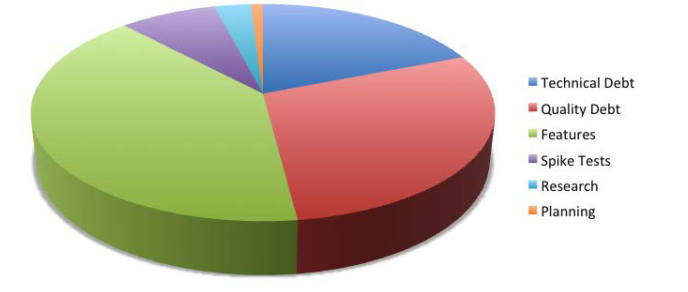
\includegraphics[width=0.5\linewidth]{visualisations/td-options.png}
	\caption{A partitioning example of work effort, provided by Cisco System's Agile Office}
	\label{fig:td-options}
\end{figure}

Similar to previous stages of technical debt, management is no easy feat.
Project managers must balance the work effort, costs with benefits, future
technical impact and return on investment. This can only be possible if
technical debt is visibile during software evolution \cite{Lim2012}
\cite{Morgenthaler2012} \cite{Codabux2013}, is continously tracked and managed
appropriately \cite{Cunningham1993}.

%%%%%%%%%%%%%%%%%%%%%%%%%%%%%%%%%%%%%%%%%%%%%%%%%%%%%%%%%%%%%%%%%%%
\subsection{Conclusion}

Technical debt is a difficult phenomenon to tackle in software engineering.
Development teams face challenges in identifying, tracking, managing and
explaining the concept to non-technical stakeholders. However, new tools allow
the indentification of code smells, tracking and computing of complex indexes
with focus on quality characteristics of code.

%%%%%%%%%%%%%%%%%%%%%%%%%%%%%%%%%%%%%%%%%%%%%%%%%%%%%%%%%%%%%%%%%%%
\section{Proposed Approach}

As mentioned, in the introduction, this study is focused on finding the relation
between technical debt and work effort. This will yeild more information for
developers on time management, for project managers on debt investment and for
stakeholders on understanding a technical concept in terms of labour cost.

The approach for this study will consist of the following steps:
\begin{enumerate}
	\item \textit{Identify appropriate data candidates for this study}.\\
	These are potential software projects that are suitable for study. At best,
	they should have multiple developers contributing to the project, a medium
	to large codebase with a variety of historical data and an associated issue
	tracking software. Ideally, the team would have integrated a continous code
	quality tool for tracking code smells throughout software evolution. This
	would help with quick and automatic identification of present and historical
	code issues. 
	
	The study would also benefit from a mixture of open-source and
	commercial sofware to contrast the differences between the two environments
	and, possibly, arrive at general conclusions that may apply to both worlds.

	\item \textit{Identify suitable work items from issue tracker}.\\
	In this step, the purpose is to understand important events in the evolution
	of the data candidates. Ideally, events were tracked in the form of tickets
	with detailed information attached, such as:
	\begin{itemize}
		\item Priority. 
		\item Estimated Work Effort.
		\item Timestamps.
		\item Assignee.  
	\end{itemize}

	This type of information would give an idea of the type of work involved.
	Unfortunately this data is not always available. The most important is the
	estimated work field as without it, the extra work cannot be identified. If
	this field does not exist in the ticket, the work item will not be included
	in the study.

	\item \textit{Identify version control checkpoints}.\\
	Successfully completed work items can be tracked in the version control
	repository of the project. Identifying checkpoints will aid in understanding
	the amount of effort put into the work item by the team and how it diverges
	from the initial estimation. 

	Ideally, the team should have links between revisions of the codebase and
	the work item in the issue tracker. This would make it easier to find the
	associated checkpoints.

	\item \textit{Measure the amount of work effort for each work item}.\\
	The purpose is to understand how many practical changes a work item has
	induced over its lifetime. This could be done in two ways: at the code and
	issue tracker levels.
	
	At the code level, it is possible to understand the level of work effort
	involved by aggregating the number of changes a work item has suffered. A
	change set consists of the number of lines of code added, deleted and
	modified. Granularity can be at the pull request, commit, class and method
	level. Version control systems such as Git provide features of retrieving
	change sets between revisions.
	
	However, identifying work effort from change sets is a challenging task. It
	is difficult to quantify in man-hours since many changes may be generated
	automatically by modern refactoring tools in the integrated development
	environment. An alternative solution is to compare the timestamps between
	the first and the last commit. The temporal difference might provide a
	practical estimate of work effort to resolve the issue. Unfortunately, this
	case only works when a developer works on a single issue at a time.

	At the ticket level, one can understand the amount of work effort realised
	by a team member. In an ideal case, the team enforces developers to log
	their time spent designing and implementing a feature. However, that is not
	always the case. An alternative option, would be to retrieve the timestamp
	of ticket events, such as the opening and closing of an issue.
	Unfortunately, this might not give an approximate time of work since: 
	\begin{itemize}
		\item The team does not respect the opening and closing of a ticket time
		according to their development patterns. For example, a developer might
		start work on an issue before marking it as "In Progress". This will
		introduce a margin of error in the estimation process.
		\item Tickets might remain open for a long period of time, whilst the
		feature was implemented in a relatively short time. Therefore this
		option would give an incorrect estimate of the amount of work completed.
		\item There are differences between commercial and open-source software.
		For example, developers might work in the timeframe of 9AM to 6PM in
		commercial environment whilst in open-source they are free to work at
		any time of the day. For example, in the extreme case, a developer marks
		a ticket as "In Progress" before end of working day, and resume the work
		the following morning. In this case, our estimation of approximately 15
		hours of development time for this work item would be incorrect.
	\end{itemize}

	It would be interesting to gather results from both methods and see how they
	correlate. Additionally, the two result sets may complement one another and
	provide an overall effort metric. However, there are many complexities and
	cases that will need to be managed to get the real estimate. 

	\item \textit{Measure technical debt items}. The scope of this step is to
	identify code violations within change sets. For each work item implemented
	there will be a set of associated modules, classes and methods affected.
	
	These will be the search areas for code smells. Using a continous code
	quality tool, historical code smells can be tracked against the evolution of
	software. If enough data is available, then patterns surrounding feature
	implementation and bug fixing can be identified.

	\item \textit{Analysis and discussion of results}.\\
	Once all previous steps have been fulfilled, the three data source must be
	linked together.

\end{enumerate}

Assumptions:
\begin{itemize}
	\item The team uses Git for version control and follows pull request model
	for implementing changes.
	\item The team uses an issue tracker consistently. Developers change the
	status of the ticket according to their current development progress. For
	example, if a team member got started on a work item, she would set the the
	ticket status to "In Progress". Respectively, she would mark the ticket as
	"Closed" if development ceased, her changes were reviewed and integrated
	into the main branch.
	\item Time?
\end{itemize}

Limitations of the study:
\begin{itemize}
	\item Data candidates
	\item Errors in ticket estimations
	\item Work effort measurement
	\item Code quality tools
	\item Assumptions
	\item Complexities of technical debt
\end{itemize}

%%%%%%%%%%%%%%%%%%%%%%%%%%%%%%%%%%%%%%%%%%%%%%%%%%%%%%%%%%%%%%%%%%%
\section{Work Plan}

show how you plan to organize your work, identifying intermediate deliverables
and dates.\\
\textbf{TBD}

%%%%%%%%%%%%%%%%%%%%%%%%%%%%%%%%%%%%%%%%%%%%%%%%%%%%%%%%%%%%%%%%%%%
\section{Conclusion}

Does it clearly explain the problem? Does it contain a bibliography and proper
citations?

Report: Is the report complete, well-organised, clear, and literate? Overall:
What is your overall impression of the student’s work?

%%%%%%%%%%%%%%%%%%%%%%%%%%%%%%%%%%%%%%%%%%%%%%%%%%%%%%%%%%%%%%%%%%%
% it is fine to change the bibliography style if you want
\pagebreak
\bibliographystyle{plain}
\bibliography{mprop}
\end{document}
